%% Beispiel-Präsentation mit LaTeX Beamer im KIT-Design
%% entsprechend den Gestaltungsrichtlinien vom 1. August 2020
%%
%% Siehe https://sdqweb.ipd.kit.edu/wiki/Dokumentvorlagen

%% Beispiel-Präsentation
\documentclass[navbaroff,en]{sdqbeamer} 
 
%% Titelbild
\titleimage{banner_2020_kit}

%% Gruppenlogo
\grouplogo{}

%% Gruppenname
\groupname{IPD - Lehrstuhl Programmierparadigmen}

% Beginn der Präsentation

\title{Vorstellung Compiler - Gruppe 3}
\subtitle{Compiler-Praktikum WS21/22}
\author[Nikolai, Pascal, Lars, Niklas]{Nikolai Maas, Pascal Mehnert, Lars König, Niklas Betten}

\date[10.\,2.\,2022]{10. Februar 2022}


\begin{document}

%Titelseite
\KITtitleframe

%Inhaltsverzeichnis
\begin{frame}{Structure}
\tableofcontents
\end{frame}

\begin{frame}
    \frametitle{Überblick}

    \begin{itemize}
        \item Compiler-Phasen
    \end{itemize}

\end{frame}


\section{Front End}

\begin{frame}
	\frametitle{Parser}

    \begin{itemize}
        \item Pull-Parser
        \item SLL(3)
        \item Precedence Climber für Expressions
        \item nicht wiederaufsetzend (keine Ankermengen)
        \item Streaming
        \item AST hierarchy with enums for selected node types
    \end{itemize}

\end{frame}

\begin{frame}
    \frametitle{Semantische Analyse}

    \begin{itemize}
        \item supports multiple errors
        \vspace{1em}
        \item Namespace Gathering
        \begin{itemize}
            \item name(space) collection
            \item exactly one main
        \end{itemize}
        \item Name / Type Analysis
        \begin{itemize}
            \item find declarations
            \item type checking
            \item expression result type
            \item duplicate variable declaration
            \item no this in static methods
            \item System-Library
        \end{itemize}
        \item Semantic Checks
        \begin{itemize}
            \item return statements
            \item keine args in main verwendet
            \item String nicht mit new erzeugt
            \item L-value assignments
            \item no pure expression statements
        \end{itemize}
    \end{itemize}

\end{frame}

\begin{frame}
    \frametitle{Transformation}

    \begin{itemize}
        \item AST -> Firm graph
        \item visitor based
        \item generation of firm types (naive)
        \item basic blocks
        \item resolve assignments
        \item boolean internal vs. value
        \item Div/Mod special case
        \item unsigned array index (undefined behavior)
    \end{itemize}

\end{frame}


\section{Middle End}

\begin{frame}
    \frametitle{Optimizations}

    \begin{itemize}
        \item bottom-up durch den call graph
        \item dead function elimination
        \item übergeordnete Fixpunkt-Iteration(en)
        \item lokale und globale Optimierungen
        \item teilweise aufgeteilt in Analyse + Umsetzung
        \vspace{1em}
        \item Constant Propagation
        \item Linear Blocks
        \item Arithmetic Identities
        \item Arithmetic Strength Reduction
        \item Pure Functions
        \item Inliner
        \item Loop Invariant Code Motion
        \item Loop Unrolling
        \item (Load/Store)
        \item (CSE)
        \item (Unused Arguments)
    \end{itemize}

\end{frame}

\begin{frame}
    \frametitle{Linear Blocks}

    \begin{itemize}
        \item remove trivial jumps
        \item join blocks with one predecessor / successor
        \item cond with equal successors (without phis)
    \end{itemize}

\end{frame}

\begin{frame}
    \frametitle{Arithmetic Strength Reduction}

    \begin{itemize}
        \item replace div / mod
        \item replace some multiplications
        \item (in general: instruction set / processor dependent)
    \end{itemize}

\end{frame}

\begin{frame}
    \frametitle{Pure Functions}

    \begin{itemize}
        \item pure -> kein Schreibzugriff auf Speicher
        \item const -> auf kein Lesezugriff auf Speicher (no mem)
        \item Termination (Rekursion, Schleife)
        \item returns newly allocated memory
        \item remove unused pure functions (incl. alloc)
    \end{itemize}

\end{frame}

\begin{frame}
    \frametitle{Inliner}

    \begin{itemize}
        \item constant arguments
        \item inside loop -> high prio
        \item code size change (factor [global] + abs [per func])
    \end{itemize}

\end{frame}

\begin{frame}
    \frametitle{Loop Invariant Code Motion}

    \begin{itemize}
        \item flat loops
        \item move to loop entry point dominator
        \item unconditional execution of moved nodes
        \item minimize reg pressure für cheap nodes
        \begin{itemize}
            \item delta loop in edges
            \item move distance
            \item number of invariant successors
        \end{itemize}
    \end{itemize}

\end{frame}

\begin{frame}
    \frametitle{Loop Unrolling}

    \begin{itemize}
        \item bottom-up through loop forest
        \item loop header format: compare const and phi (const init + backedges [add with const])
        \item max abs number of unrolled iterations
        \item loop body size
        \item complete unroll -> larger size allowed
    \end{itemize}

\end{frame}

\begin{frame}
    \frametitle{Unused Arguments}

    \begin{itemize}
        \item incl. in recursive calls (fix-point analysis)
    \end{itemize}

\end{frame}


\section{Backend}

\begin{frame}
    \frametitle{Intermediate Language}

    \begin{itemize}
        \item close to x86-64 assembler
        \item virtual registers
        \item phis can be assigned to basic blocks -> resolved later
        \item additional virtual instructions (div / mod / call)
    \end{itemize}

\end{frame}

\begin{frame}
    \frametitle{Instruction Selection}

    \begin{itemize}
        \item bottom-up pattern matching -> single pattern per node
        \item no cost function
        \item bottom-up pattern collection (postorder on matched patterns -> ignores unnecessary predecessor patterns)
        \item topological order of instructions
        \item virtual registers
        \item basic and advanced patterns (add: add r r, addi r, add r i, lea)
        \item register restrictions not considered
        \item separate phi resolving phase
        \item memory dependencies discarded
        \vspace{1em}
        \item no separate instruction scheduling
    \end{itemize}

\end{frame}

\begin{frame}
    \frametitle{Phi Resolving}

    \begin{itemize}
        \item works on intermediate language
        \item add moves to predecessor blocks
        \item ?
        \item permutations
        \item critical edges
    \end{itemize}

\end{frame}

\begin{frame}
    \frametitle{Register Allocation - Techniques}

    \begin{itemize}
    	\item Blockwise
        \item Linear Scan
        \item Graph Coloring
    \end{itemize}

\end{frame}

\begin{frame}
\frametitle{Register Allocator - Overview}

\centering 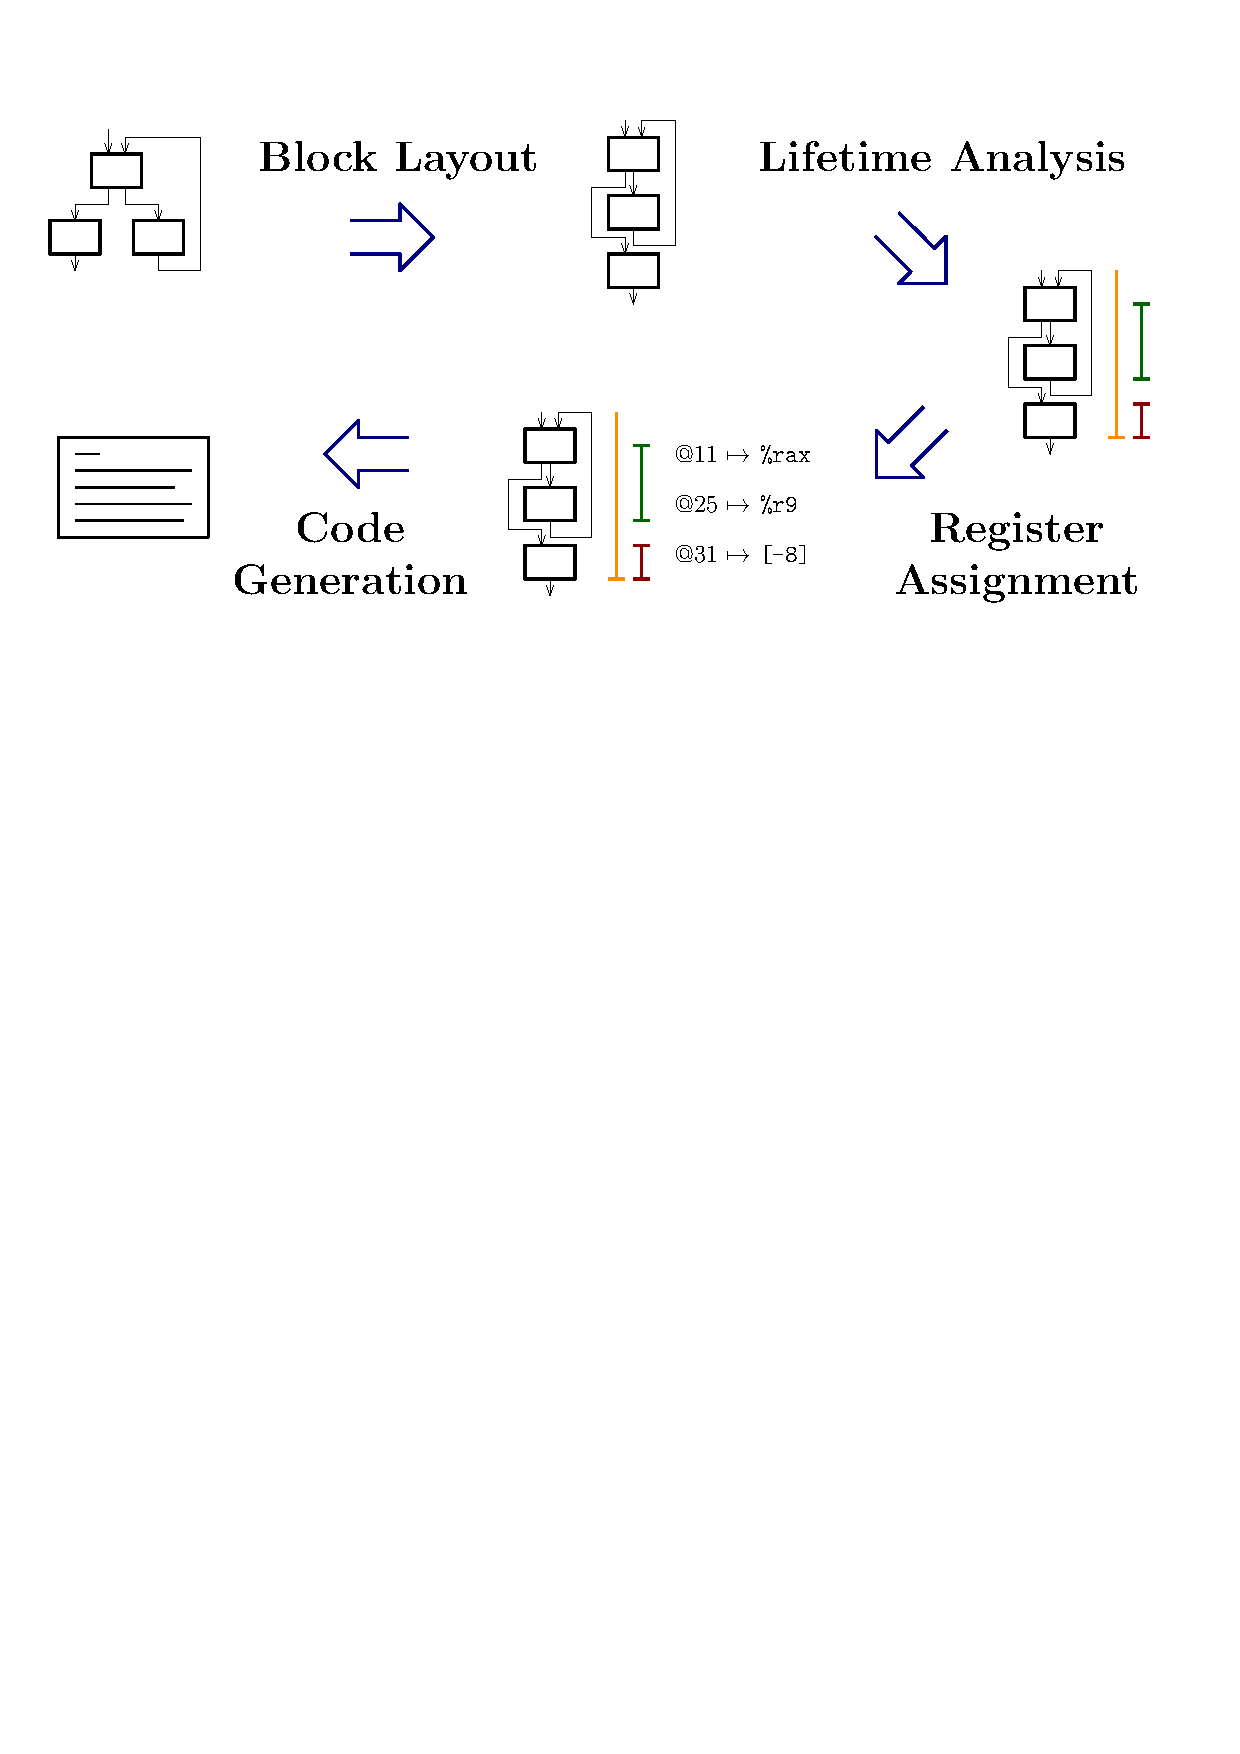
\includegraphics[scale=0.7]{images/overview.pdf}

\end{frame}

\begin{frame}
    \frametitle{Register Allocator}

    \begin{itemize}
        \item[1.] block order
        \begin{itemize}
            \item topological (reverse postorder, control flow)
            \item loop aware (loop blocks directly after loop header)
        \end{itemize}
        \item[2.] lifetime analysis
        \begin{itemize}
            \item linear through blocks
            \item lifetime for all virtual registers
            \item expand lifetime of variables in loops
            \item reuse register if virtual register lifetime ends as instruction argument
            \item linear lifetimes (no splits)
            \item collect additional information for register allocation heuristic (number of calls / divs, loop depth)
        \end{itemize}
    \end{itemize}

\end{frame}

\begin{frame}
    \frametitle{Register Allocator}

    \begin{itemize}
        \item[3.] register allocation
        \begin{itemize}
            \item linear scan
            \item generates mapping from virtual to processor? registers
            \item heuristic for spill decision (loop depth)
            \item spill virtual register for entire lifetime
            \item unify virtual registers / registers
            \begin{itemize}
                \item in-out virtual registers
                \item registers for call arguments (in / out)
            \end{itemize}
            \item reuse stack slots if lifetime don't overlap
        \end{itemize}
        \item[4.] code generation
        \begin{itemize}
            \item x86-64 call convetion (systemv)
            \begin{itemize}
                \item 6 arguments in register
                \item rest on stack
                \item caller / callee stacked registers
                \item efficient implementation by calculating register permutation
            \end{itemize}
            \item 16-bit alignment for stdlib calls only
            \item omit load of spilled register if temp. register is still available (inside basic blocks)
        \end{itemize}
    \end{itemize}

\end{frame}

\begin{frame}
    \frametitle{Peephole Optimizations}

    \begin{itemize}
        \item fixed-size (per optimization) window of instructions
        \vspace{1em}
        \item Jump Inversion
    \end{itemize}

\end{frame}

\begin{frame}
    \frametitle{Assembly Output}

    \begin{itemize}
        \item ELF file format
        \item function prologs / epilogs
        \item link runtime library (written in C)
        \item passed to gcc
    \end{itemize}

\end{frame}


\begin{frame}
\end{frame}

\appendix
\beginbackup

\backupend

\end{document}
